\documentclass[letterpaper,openright,10pt,oneside]{report}

\usepackage[spanish,activeacute]{babel}
\usepackage[utf8]{inputenc}
\usepackage[letterpaper,width=150mm,top=25mm,bottom=25mm]{geometry}
\usepackage{fancyhdr}
\usepackage{verbatim}
\pagestyle{fancy}

\fancyhead{}
\fancyhead[RO,LE]{Sistema de alertas de promociones integrando mensajeria en tiempo real}

\fancyfoot{}
\fancyfoot[LE,RO]{\thepage}
\fancyfoot[LO,CE]{Taller de Proyecto de Software}
\fancyfoot[CO,RE]{Ignacio Jara}



%Gummi|065|=)
\title{\textbf{Sistema de alertas de promociones integrando mensajeria en tiempo real}}
\author{Ignacio Jara\\Taller de Proyecto de Software\\Raúl del Canto\\INACAP Apoquindo}

\date{\today}
\usepackage{graphicx}
\begin{document}
\maketitle

\part{Propósito del documento}
	\chapter*{Resumen ejecutivo}
	Actualmente todas las empresas o personas que desean ofrecer un producto a través de internet, deben realizarlo a través de plataformas, en las que ingresan los productos y esperar a que alguien responda desde variados medios de comunicación, ya sea una llamada como un mensaje a través de correo electronico. Las empresas que desean comenzar a operar a través de internet, también se encuentran con similares dificultades, ya que ofrecer un sitio de comercio electronico tiende a ser engorroso y caro.
	

	El objetivo de este proyecto, es entregun un repositorio en el cual, organizaciones y personas naturales puedan ofrecer sus productos a través de internet. Sin intermediarios o inversiones que pueden significar un desmedro a sus negocios.
	Para lograr este objetivo, se crea un software que permite la exhibición de productos a través de ella, junto a un modulo de comunicación en tiempo real, llamado "chat", en el cual se puede llegar a un acuerdo directamente con la persona encargada en la empresa o con la personas que ofrece el producto o servicio.
	
	Todos los interesados pueden subir y ofrecer sus productos a través de los llamados "mensajes", sin embargo, existirán mensajes destacados al invertir en este.
	
	\chapter*{Objetivo del documento}
	Principalmente, en este documento se detallará el plan para formar un organización, sus necesidades y procesos, para sostener el proyecto contenido en esta tesis, que es la de formar un sistema de alertas de promociones con mensajería en tiempo real.
	
	Se detalla el alcance que tiene el proyecto, junto a las metas y objetivos que este debo cumplir para el pleno funcionamiento de la organización, se escriben los requerimientos de las empresas y personas interesadas en esta plataforma. Con estos datos es posible diagramar los procesos que realizará el software, para suplir estas necesidades, junto con el diseño de la base de datos, que guardará la información para ser utlizados en la plataforma.
	
	A su vez, se detallan los procesos que realiza la organización, como obtiene recursos, opera y reinvierte sus ganancias para mejorar sus alcance. Se especifican los roles que existen y como operan entre si, como también el modelo de negocio a seguir, detallando los potenciales riesgos que pueden aparecer durante el tiempo de vida del proyecto y los costos asociados en la creación y mantención de la plataforma.
	
	El plan de negocio entrega la respuesta a como tratar con este tipo de organizaciones, como agregar valor a nuestro producto y a las entidades interesadas en el, y detallar los puntos positivos que son necesario explotar y los puntos negativos que quedan por mejorar. Permite detallar el mercado objetivo al cual apuntamos y todos los procesos a realizar para darle forma a la organización.
	
	Luego se detallan las especificaciones del software y el hardware para el correcto funcionamiento del aplicativo, la forma en la cual los usuarios interactuarán con ella y los GAP's que puedan aparecer durante el desarrollo de esta; Se documentan los requisitos funcionales y no funcionales, ademas de los pasos a seguir usando metodología.
	
	Al finalizar el documento estan las conclusiones de este caso, que de una u otra forma, permiten comprender el significado del proyecto y las implicancias que tiene este en la sociedad.
\tableofcontents
\newpage
\part{Desripción del proyecto}
	\chapter{Marco general del proyecto}
		\section{Misión del proyecto}
		
		Proveer un sistema confiable y seguro, para que los encargados de las organizaciones y personas naturales puedan ingresar su información de contacto y ofrecer productos y /o servicios a través de nuestra plataforma. El objetivo es llegar a la mayor cantidad de personas u organizaciones que estén interesados.
		Ofrecer un servicio en la nube, para ofrecer servicios o productos, que estos se muestren en tiempo real, permitiendo a los intersados en esos servicios, adquirirlos directamente con la fuente. Sirviendo de nexo directo entre vendedor y comprador.
		\section{Lineamientos estratégicos}
			\begin{itemize}
				\item Proteger la información. \newline
					Entregar seguridad y confidencialidad en la información en la plataforma es crucial para el negocio. 
				\item Generar lazos y relaciones. \newline
				Una parte importante en todo negocio es que las empresas aprendan de sus clientes para reinventarse. La comunicación directa permite saber que piensan sus clientes y como se pueden ofrecer productos relacionados.
				\item Apoyo a todo tipo de venta. \newline
				Todas las empresas o personas naturales tienen la posibilidad de competir en iguales terminos, ofreciendo productos similares con precios seleccionados por ellos. Permitiendo una libre competencia.
			\end{itemize}
		\section{Objetivos}
			\begin{itemize}
				\item Crear un archivo que contenga la información entregada.
				\item Organizar la información de manera ordenada e intuitiva.
				\item Ofrecer un conjunto de funciones para la creación de aplicaciones.
				\item Ofrecer una plataforma de comunicación directa entre vendedores y clientes.
				\item Control de alertas y mensajes.
			\end{itemize}
		\section{Metas de gestión del proyecto}
			Indexación de toda la información relacionada entre producto, servicio, cliente y organización, para ponerla a sus disposición y alcance de ellos. Fundamentalmente se define metas para gestionar el proyecto desde el punto de vista informatico.
			\begin{enumerate}
				\item Instaurar una plataforma informatica en un plazo de 6 meses.
				\item Contactar con empresas y personas que desean ofrecer sus productos o servicios durante 1 año.
				\item Mantener el proyecto reinvirtiendo las ganancias.
				\item Después del primer año, se realizaran modificaciones al proyecto, en base a ganancias y gasto.	
			\end{enumerate}
			\chapter{Alcance del proyecto}
				\section{Dimensiones del alcance}
					Cuando nos presentamos ante cualquier proyecto, el objetivo es definir el alcance o el impacto que este tiene en el medio en el cual será insertado, para ello, es necesario definir limites que delimitan el actuar del proyecto y lo que puede o no hacer. Esto ayuda a enfocar los esfuerzos en la problematica en sí y no desviarse del objetivo principal.
					\subsection{Empresarial}
						\begin{itemize}
							\item La organización será con fines de lucro.
							\item Su base de operaciones será en Santiago, Región Metropolitana, Chile.
							\item Se encriptará la información contenida en la plataforma.
							\item Los interesados en mejorar la plataforma, pueden acceder a una api para manejar los datos.
							\item El proceso para registrar una aplicacion relacionada, requiere pasar un proceso fisico de aceptación a la empresa o persona en cuestión.
						\end{itemize}
					\subsection{Funcional}
						\begin{itemize}
							\item Se contactarán organizaciones en la región
							\item Se contactarán a personas naturales o con giro comercial en la región.
							\item Para ser una organización certificada en el aplicativo, debe pasar un proceso de aceptación.
							\item Los datos serán guardados en una base de datos radicada en Chile.
\end{itemize}
					\subsection{Principal - Core}
						\begin{itemize}
							\item Esta información solo será accesible por clientes, organizaciones y administradores de la plataforma.
							\item Se entregará información en tiempo real, generada en la plataforma.
							\item Los datos serán almacenados en una base de datos NoSQL.
							\item La interfaz será via Web.
							\item La aplicación y documentación estará en idioma español.
						\end{itemize}
				\section{Solución propuesta}
				La solución propuesta es proveer una base de datos no relacional, donde se almacenarán los datos de los clientes y las organizaciones que deseen formar parte del proyecto. La información almacenada se entregará en tiempo real a los clientes, por lo cual, se puede manejar la información de manera intuitiva y eficaz. Se proveera una interfaz web.
					\subsection{Ambito financiero}
						\begin{itemize}
							\item La plataforma será de acceso gratuito para clientes y personas naturales.
							\item La plataforma colocará un distintivo a los mensajes pertenecientes a organizaciones certificadas.
							\item Existirá publicidad que proveen terceros.
						\end{itemize}
					\subsection{Ambito de operaciones}
						\begin{itemize}
							\item Los datos serán almacenados en un VPS ubicado en Chile.
							\item Se generarán mensajes.
							\item Se proveerá un sistema de mensajes en tiempo real.
							\item Se almacenará información sensible\footnote{Detallada en la ley 19.628} sobre los usuarios.
							\item Se almacenará información sensible sobre las organizaciones que forman parte. 
						\end{itemize}
					\subsection{Ambito de Recursos Humanos(HR)}
						\begin{itemize}
							\item Se contratará a un Informatico para la programación y puesta en marcha.
							\item Se contratarán a personas dedicas a administrar y promover la aplicación.
							\item Se contratará a un Informatico para la mantención de la plataforma.
							\item Los sueldos se reajustarán en base a proyecciones, apital y legislación vigente, de manera anual.
						\end{itemize}
					\subsection{Ambito anal'itico}
						\begin{itemize}
							\item Modulos sistema:
								\subitem Guardado de datos: Se reciben los datos en formato JSON y son ingresados en la Base de Datos.
								\subitem Entrega de información: Los datos serán entregados en formato JSON al aplicativo.
							\item Modulos Plataforma WEB
								\subitem Información General
									\subsubitem Información de la organización: Aquí se datallan los datos de la organización.
								\subitem Usuario Registrado
									\subsubitem Muestra de datos: La información se muestra en formato HTML\footnote{lenguaje de marcas de hipertexto} para su lectura.
								\subitem Modulo de Mensajes
									\subsubitem Inserción de Mensajes
									\subsubitem Borrado de Mensajes
									\subsubitem Detalle de Mensajes
								\subitem Modulo de Chat
									\subsubitem Creación de sala de chat
									\subsubitem Listado de Chats
						\end{itemize}
				\section{Marco de Alcance}	
						\subsection{Supuestos}
							\begin{itemize}
								\item El sistema estará basado en CLOUD.
								\item La plataforma será accesible 24/7/365.
								\item Se proveerá una aplicación WEB para el acceso a los datos.
								\item La administración solo será accesible para personal autorizado.
								\item Solo entidades certificadas y clientes podran operar los datos.
								\item Solo existe un/a encargado por organización que pueda acceder a la plataforma.
								\item Los datos estarán encriptados dentro de la base de datos.
							\end{itemize}
						\subsection{Exclusiones}
							\begin{itemize}
								\item La empresa no se hace responsable por fraudes o situaciones legales.
								\item La empresa entregará toda la información relevante a autoridades sobre el tema.
								\item La mesa de ayuda solo funcionará en horario de oficina.
								\item No se verifican cambios en los datos de las organizaciones ni clientes.
							\end{itemize}
\part{Modulos}
\section{Casos de uso}
	En forma general, cada usuario pueden acceder a distintos modulos de la aplicación
	\begin{figure}[htp]
\centering
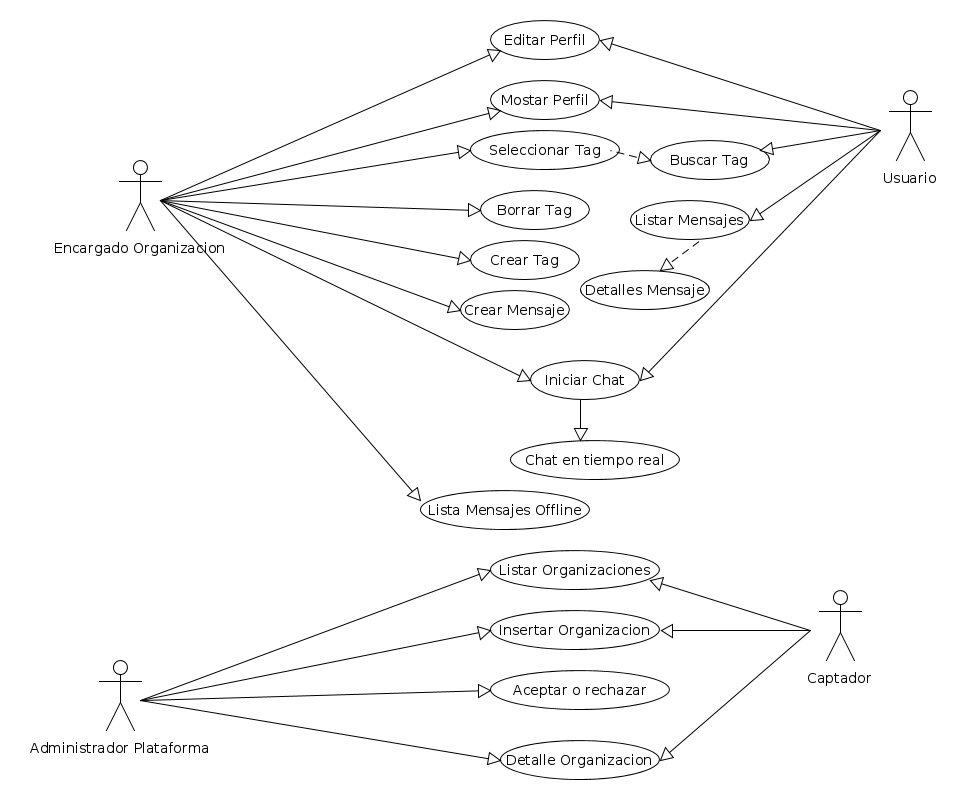
\includegraphics[scale=0.40]{/home/ijara/Dropbox/TESIS/Diagramas/casosdeuso.png}
\caption{Casos de Uso}

\label{}\end{figure}\newpage
\section{Detalle casos de uso}
\subsection{Editar Perfil}

\begin{tabular}{|c|p{110mm}|}
\hline
	Caso de uso & Editar Perfil\\
\hline
	Resumen & Modulo para la edición del item perfil, en el cual,
	usuarios y organizaciones pueden diferenciarse y colocar información personal\\
\hline
	Actor & Encargado organizacion, Usuario\\
\hline
	Precondición & Registrado en el sistema\\
\hline
	Descripción & 
	\underline{Trayectoria Basica}
	\begin{itemize}
		\item el actor selecciona opcion editar perfil
		\item el actor recibe formulario
		\item el actor completa los datos del formulario
		\item el actor selecciona guardar
		\item el actor recibe mensaje de exito
	\end{itemize}
	\underline{Trayectoria alterna}
	\begin{itemize}
		\item el actor selecciona cancelar
		\item el actor vuelve a la pagina anterior
	\end{itemize}\\
\hline
	Postondición & el actor recibe mensaje\\
\hline
\end{tabular}

\subsection{Mostrar Perfil}

\begin{tabular}{|c|p{110mm}|}
\hline
	Caso de uso & Mostrar Perfil\\
\hline
	Resumen & Pagina que detalla el perfil actual del actor\\
\hline
	Actor & Encargado organizacion, Usuario\\
\hline
	Precondición & Registrado en el sistema\\
\hline
	Descripción & 
	\underline{Trayectoria Basica}
	\begin{itemize}
		\item el actor selecciona opcion mostrar perfil
		\item el actor recibe pagina con el detalle de su perfil
	\end{itemize}
	\\
\hline
	Postondición & el actor recibe pagina\\
\hline
\end{tabular}

\subsection{Seleccionar Tag}

\begin{tabular}{|c|p{110mm}|}
\hline
	Caso de uso & Seleccionar Tag\\
\hline
	Resumen & Modulo para la seleccion de un tag que relaciona un tema con la organizacion o usuario\\
\hline
	Actor & Encargado organizacion, Usuario\\
\hline
	Precondición & Registrado en el sistema\\
\hline
	Descripción & 
	\underline{Trayectoria Basica}
	\begin{itemize}
		\item el actor selecciona opcion seleccionar tag
		\item el actor recibe formulario con opciones a elegir
		\item *ver caso de uso Buscar Tag*
		\item el actor completa los datos del formulario
		\item el actor selecciona guardar
		\item el actor recibe mensaje de exito
	\end{itemize}
	\underline{Trayectoria alterna}
	\begin{itemize}
		\item Encargado organizacion
		\item el actor no encuentra un tag apropiado
		\item el actor selecciona crear tag
		\item *ver caso de uso Crear Tag*
	\end{itemize}\\
\hline
	Postondición & el actor recibe mensaje de exito\\
\hline
\end{tabular}

\subsection{Buscar Tag}

\begin{tabular}{|c|p{110mm}|}
\hline
	Caso de uso &  Buscar Tag\\
\hline
	Resumen & Modulo para la busqueda de tags en la base de datos\\
\hline
	Actor & Encargado organizacion, Usuario\\
\hline
	Precondición & Registrado en el sistema\\
\hline
	Descripción & 
	\underline{Trayectoria Basica}
	\begin{itemize}
		\item el actor recibe formulario
		\item el actor escribe caracteres en formulario
		\item el actor recibe tags que contienen estos caracteres
		\item el actor selecciona el tag buscado
		\item el actor repite el proceso hasta seleccionar todos los tags buscados
		\item el actor selecciona opcion guardar
	\end{itemize}
	\underline{Trayectoria alterna}
	\begin{itemize}
		\item Encargado Organizacion
		\item el actor no encuentra un tag apropiado
		\item el actor el actor selecciona crear tag
		\item *ver casp de uso Crear Tag* 
	\end{itemize}\\
\hline
	Postondición & el actor recibe mensaje de exito\\
\hline
\end{tabular}

\subsection{Borrar Tag}

\begin{tabular}{|c|p{110mm}|}
\hline
	Caso de uso & Borrar Tag\\
\hline
	Resumen & Modulo para la quitar la relacion entre organizacion y un tag\\
\hline
	Actor & Encargado organizacion\\
\hline
	Precondición & Registrado en el sistema\\
\hline
	Descripción & 
	\underline{Trayectoria Basica}
	\begin{itemize}
		\item el actor selecciona borrar tag
		\item el actor recibe tabla con todos los tags relacionados
		\item el actor selecciona borrar tag en la tabla
		\item el actor recibe mensaje de exito
	\end{itemize}
	\underline{Trayectoria alterna}
	\begin{itemize}
		\item el actor selecciona cancelar
		\item el actor vuelve a la pagina anterior
	\end{itemize}\\
\hline
	Postondición & el actor recibe mensaje de exito\\
\hline
\end{tabular}

\subsection{Crear Tag}

\begin{tabular}{|c|p{110mm}|}
\hline
	Caso de uso & Crear Tag\\
\hline
	Resumen & Modulo para la creacion de tag\\
\hline
	Actor & Encargado organizacion\\
\hline
	Precondición & Registrado en el sistema\\
\hline
	Descripción & 
	\underline{Trayectoria Basica}
	\begin{itemize}
		\item el actor selecciona opcion crear tag
		\item el actor recibe formulario
		\item el actor completa los datos del formulario
		\item el actor selecciona guardar
		\item el actor recibe mensaje de exito
	\end{itemize}
	\underline{Trayectoria alterna}
	\begin{itemize}
		\item el actor selecciona cancelar
		\item el actor vuelve a la pagina anterior
	\end{itemize}\\
\hline
	Postondición & el actor recibe mensaje de exito\\
\hline
\end{tabular}

\subsection{Crear Mensaje}

\begin{tabular}{|c|p{110mm}|}
\hline
	Caso de uso & Crear Mensaje\\
\hline
	Resumen & Modulo para la creación de mensaje promocional en la plataforma\\
\hline
	Actor & Encargado organizacion\\
\hline
	Precondición & Registrado en el sistema\\
\hline
	Descripción & 
	\underline{Trayectoria Basica}
	\begin{itemize}
		\item el actor selecciona opcion crear mensaje
		\item el actor recibe formulario
		\item el actor completa los datos del formulario
		\item el actor selecciona guardar
		\item el actor recibe mensaje de exito
	\end{itemize}
	\underline{Trayectoria alterna}
	\begin{itemize}
		\item el actor selecciona cancelar
		\item el actor vuelve a la pagina anterior
	\end{itemize}\\
\hline
	Postondición & el actor recibe mensaje de exito\\
\hline

\end{tabular}

\subsection{Listar Mensajes}

\begin{tabular}{|c|p{110mm}|}
\hline
	Caso de uso & Listar Mensajes\\
\hline
	Resumen & Modulo principal donde aparecen los mensajes relacionados al tag del usuario\\
\hline
	Actor & Usuario\\
\hline
	Precondición & Registrado en el sistema\\
\hline
	Descripción & 
	\underline{Trayectoria Basica}
	\begin{itemize}
		\item el actor accede a la pagina principal
		\item el actor recibe listado de mensajes relacionados al tag
	\end{itemize}
	\\
\hline
	Postondición & el actor recibe pagina\\
\hline
\end{tabular}
\subsection{Detalles Mensaje}

\begin{tabular}{|c|p{110mm}|}
\hline
	Caso de uso & Detalles Mensaje\\
\hline
	Resumen & Modulo para la edición del item perfil, en el cual,
	usuarios y organizaciones pueden diferenciarse y colocar información personal\\
\hline
	Actor & Usuario\\
\hline
	Precondición & Caso de uso Listar Mensajes\\
\hline
	Descripción & 
	\underline{Trayectoria Basica}
	\begin{itemize}
		\item el actor selecciona un mensaje
		\item el actor recibe una pagina con el detalle
	\end{itemize}
	\underline{Trayectoria alterna}
	\begin{itemize}
		\item el actor selecciona opcion cerrar
		\item el actor vuelve a la lista de mensajes
	\end{itemize}\\
\hline
	Postondición & el actor recibe pagina\\
\hline
\end{tabular}
\subsection{Iniciar Chat}

\begin{tabular}{|c|p{110mm}|}
\hline
	Caso de uso & Iniciar Chat\\
\hline
	Resumen & Modulo para el sistema de mensajeria en tiempo real\\
\hline
	Actor & Encargado organizacion, Usuario\\
\hline
	Precondición & Registrado en el sistema, usuario en detalle mensaje\\
\hline
	Descripción & 
	\underline{Trayectoria Basica}
	\begin{itemize}
		\item encargado organizacion selecciona opcion chat
		\item encargado recibe pagina con sistema de mensajeria
		\item usuario selecciona opcion chat
		\item actores se conectan a una sala de chat con el titulo del mensaje
	\end{itemize}
	\underline{Trayectoria alterna}
	\begin{itemize}
		\item el actor selecciona abandonar chat
		\item el actor vuelve a la pagina anterior
	\end{itemize}\\
\hline
	Postondición & los actores abandonan la sala de chat\\
\hline
\end{tabular}

\subsection{Chat en tiempo real}

\begin{tabular}{|c|p{110mm}|}
\hline
	Caso de uso &  Chat en tiempo real\\
\hline
	Resumen & Modulo que detalla la comunicación en tiempo real\\
\hline
	Actor & Encargado organizacion, Usuario\\
\hline
	Precondición & Registrado en el sistema, caso de uso iniciar chat\\
\hline
	Descripción & 
	\underline{Trayectoria Basica}
	\begin{itemize}
		\item el actor envia mensaje
		\item el actor recibe lista de mensajes
	\end{itemize}
	\underline{Trayectoria alterna}
	\begin{itemize}
		\item el actor selecciona abandonar chat
		\item el actor vuelve a la pagina anterior
	\end{itemize}\\
\hline
	Postondición & los actores abandonan la sala de chat\\
\hline
\end{tabular}

\subsection{Lista Mensajes Offline}

\begin{tabular}{|c|p{110mm}|}
\hline
	Caso de uso & Lista Mensajes Offline\\
\hline
	Resumen & Modulo para obtener listado de conversaciones almacenados en el sistema\\
\hline
	Actor & Encargado organizacion\\
\hline
	Precondición & Registrado en el sistema, al menos un chat realizado con exito\\
\hline
	Descripción & 
	\underline{Trayectoria Basica}
	\begin{itemize}
		\item el actor selecciona listar mensajes offline
		\item el actor tabla con datos de mensajes
		\item el actor selecciona mensaje
		\item el actor recibe el detalle de la conversación
	\end{itemize}
	\underline{Trayectoria alterna}
	\begin{itemize}
		\item el actor selecciona cancelar
		\item el actor vuelve a la pagina anterior
	\end{itemize}\\
\hline
	Postondición & el actor recibe detalle de conversación\\
\hline
\end{tabular}

\subsection{Listar Organizaciones}

\begin{tabular}{|c|p{110mm}|}
\hline
	Caso de uso & Listar Organizaciones\\
\hline
	Resumen & Modulo para mostrar el listado de organizaciones que estan interesadas en ingresar el sistema\\
\hline
	Actor & Administrador plataforma, Captador\\
\hline
	Precondición & Registrado en el sistema, Existen organizaciones interesadas\\
\hline
	Descripción & 
	\underline{Trayectoria Basica}
	\begin{itemize}
		\item el actor selecciona opcion Listar organizaciones
		\item el actor recibe tabla con información basica de organizaciones
		\item el actor selecciona una organizacion
		\item el actor recibe detalle de la organizacion
	\end{itemize}
	\underline{Trayectoria alterna}
	\begin{itemize}
		\item el actor selecciona cancelar
		\item el actor vuelve a la pagina anterior
	\end{itemize}\\
\hline
	Postondición & caso de uso detalle organizacion\\
\hline
\end{tabular}


\subsection{Insertar Organizacion}

\begin{tabular}{|c|p{110mm}|}
\hline
	Caso de uso & Insertar Organizacion\\
\hline
	Resumen & Modulo para la inserción de organizaciones pendientes de confirmación de ingreso\\
\hline
	Actor & Administrador Plataforma, Captador\\
\hline
	Precondición & Registrado en el sistema, existe organizacion interesada\\
\hline
	Descripción & 
	\underline{Trayectoria Basica}
	\begin{itemize}
		\item el actor selecciona insertar organizacion
		\item el actor recibe formulario
		\item el actor completa los datos del formulario
		\item el actor selecciona guardar
		\item el actor recibe mensaje de exito
	\end{itemize}
	\underline{Trayectoria alterna}
	\begin{itemize}
		\item el actor selecciona cancelar
		\item el actor vuelve a la pagina anterior
	\end{itemize}\\
\hline
	Postondición & el actor recibe mensaje de exito\\
\hline
\end{tabular}

\subsection{Aceptar o Rechazar}

\begin{tabular}{|c|p{110mm}|}
\hline
	Caso de uso & Aceptar o Rechazar\\
\hline
	Resumen & Modulo para aceptar o rechazar el ingreso al sistema de una organizacion determinada\\
\hline
	Actor & Administrador plataforma\\
\hline
	Precondición & Registrado en el sistema, caso de uso detalle organizacion\\
\hline
	Descripción & 
	\underline{Trayectoria Basica}
	\begin{itemize}
		\item el actor recibe detalle organizacion
		\item el actor recibe documentacion asociada
		\item el actor selecciona aceptar
		\item se envia mensaje a la organización
	\end{itemize}
	\underline{Trayectoria alterna}
	\begin{itemize}
		\item el actor selecciona rechazar
		\item se envia mensaje a la organización
		\item el actor vuelve a la pagina anterior
	\end{itemize}\\
\hline
	Postondición & el sistema envia mensaje a organización\\
\hline

\end{tabular}
\subsection{Detalle organización}

\begin{tabular}{|c|p{110mm}|}
\hline
	Caso de uso & Detalle organización\\
\hline
	Resumen & Modulo que inserta detalles y documentación de la organización\\
\hline
	Actor & Administrador plataforma, Captador\\
\hline
	Precondición & Registrado en el sistema, se ha insertado organizacion, caso de uso listar organizaciones\\
\hline
	Descripción & 
	\underline{Trayectoria Basica}
	\begin{itemize}
		\item el actor selecciona opcion detalle organizacion
		\item el actor recibe formulario
		\item el actor completa los datos del formulario
		\item el actor selecciona guardar
		\item el actor recibe mensaje de exito
	\end{itemize}
	\underline{Trayectoria alterna}
	\begin{itemize}
		\item el actor selecciona cancelar
		\item el actor vuelve a la pagina anterior
	\end{itemize}\\
\hline
	Postondición & el actor recibe mensaje de exito\\
\hline
\end{tabular}
\chapter{Diagrama de Componentes}
\section{Diagrama de componentes de software}
Se utilizará metodología Modelo - Vista - Controlador, para separar la parte logica con las vistas de la aplicación. Entregar mayor flexibilidad y seguridad a las conexiones y definiciones de la base de datos y utilizar tecnologías que permitan reutilizar codigo y una alta escalabilidad. La plataforma está formada por una base de datos no relacional, a la cual se conectaran al sistema utilizando un conector escrito en JavaScript. La plataforma correrá sobre un sistema escrito en NodeJS desde el servidor, y entregará los resultados a través de AngularJS, que junto a HTML y CSS entregarán los resultados en una pagina web. A su vez, la información puede ser enviada a través de formato json para futuras actualizaciones (sistemas transaccionales, programas propios, programas de terceros, aplicaciones web, aplicaciones moviles).
\begin{figure}[htp]
\centering
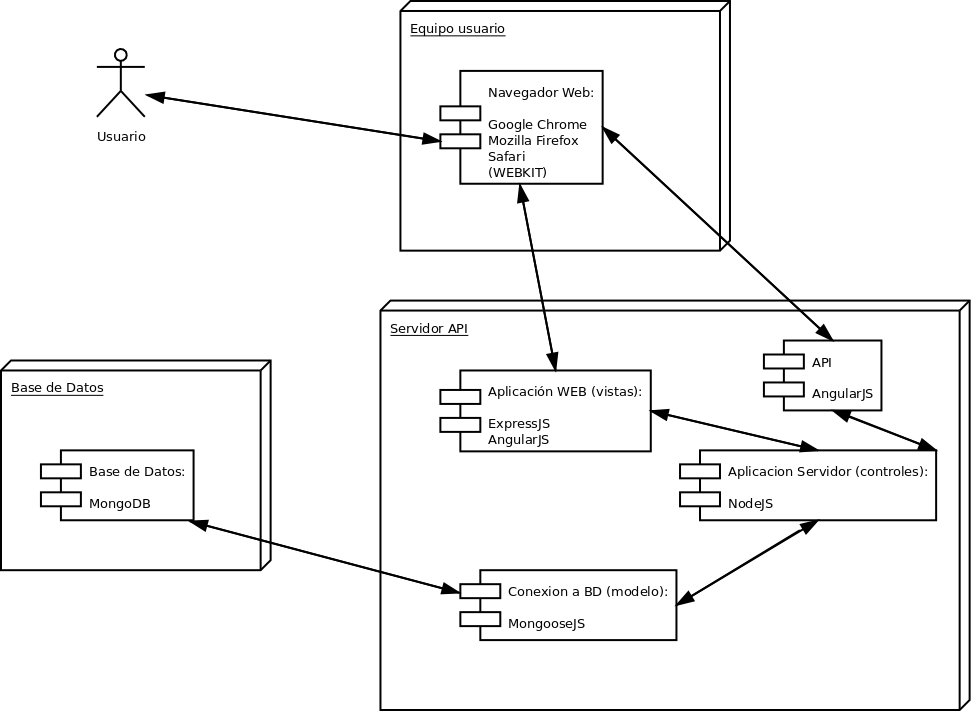
\includegraphics[scale=0.30]{/home/ijara/Dropbox/TESIS/Diagramas/componentessoftware.png}
\caption{Diagrama componentes software}
\label{}
\end{figure}
\section{diagrama de componentes de hardware}
La plataforma estará alojada en un cloud, protegida detraś de un firewall ante el acceso indebido y a través de servicios que ofrecen empresas externas para evitar ataques.
\begin{figure}[htp]
\centering
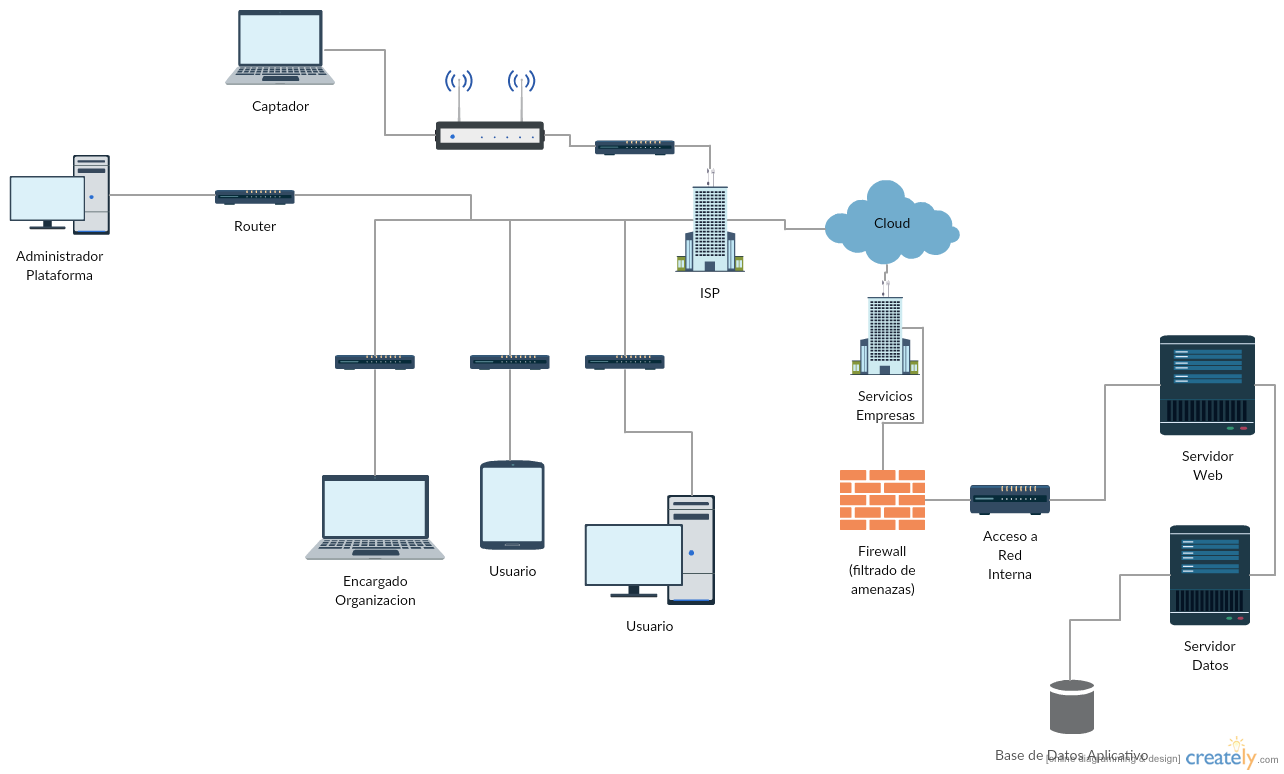
\includegraphics[scale=0.30]{/home/ijara/Dropbox/TESIS/Diagramas/diagramahardware.png}
\caption{Diagrama Componentes Hardware}
\label{}
\end{figure}
\chapter{Diagramas de Secuencia}
En este capitulo se muestran los distintos diagramas de secuencia de cada uno de los casos de uso existentes en la plataforma.
\begin{figure}[htp]
\centering
\includegraphics[scale=0.25]{/home/ijara/Dropbox/TESIS/Diagramas/diagramasdeflujo/editarperfil.png}
\caption{Editar Perfil}
\label{}
\end{figure}
\begin{figure}[htp]
\centering
\includegraphics[scale=0.25]{/home/ijara/Dropbox/TESIS/Diagramas/diagramasdeflujo/mostrarperfil.png}
\caption{Mostrar Perfil}
\label{}
\end{figure}\begin{figure}[htp]
\centering
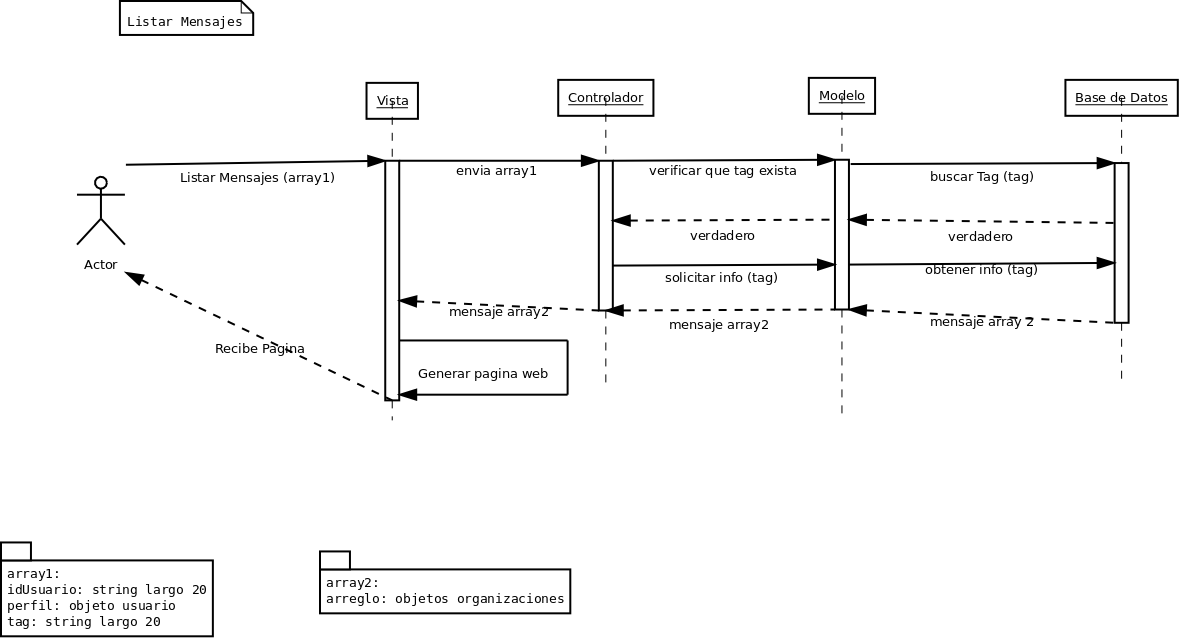
\includegraphics[scale=0.25]{/home/ijara/Dropbox/TESIS/Diagramas/diagramasdeflujo/listarMensajes.png}
\caption{Listar Mensajes}
\label{}
\end{figure}
\begin{figure}[htp]
\centering
\includegraphics[scale=0.25]{/home/ijara/Dropbox/TESIS/Diagramas/diagramasdeflujo/seleccionartag.png}
\caption{Seleccionar Tag}
\label{}
\end{figure}
\begin{figure}[htp]
\centering
\includegraphics[scale=0.25]{/home/ijara/Dropbox/TESIS/Diagramas/diagramasdeflujo/seleccionartag.png}
\caption{Buscar Tag}
\label{}
\end{figure}
\begin{figure}[htp]
\centering
\includegraphics[scale=0.25]{/home/ijara/Dropbox/TESIS/Diagramas/diagramasdeflujo/borrartag.png}
\caption{Borrar Tag}
\label{}
\end{figure}
\begin{figure}[htp]
\centering
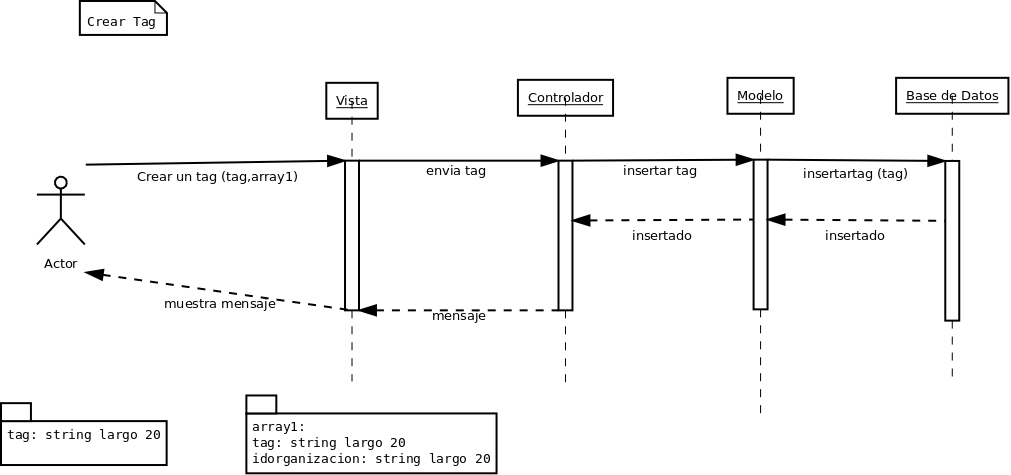
\includegraphics[scale=0.25]{/home/ijara/Dropbox/TESIS/Diagramas/diagramasdeflujo/creartag.png}
\caption{Crear Tag}
\label{}
\end{figure}
\begin{figure}[htp]
\centering
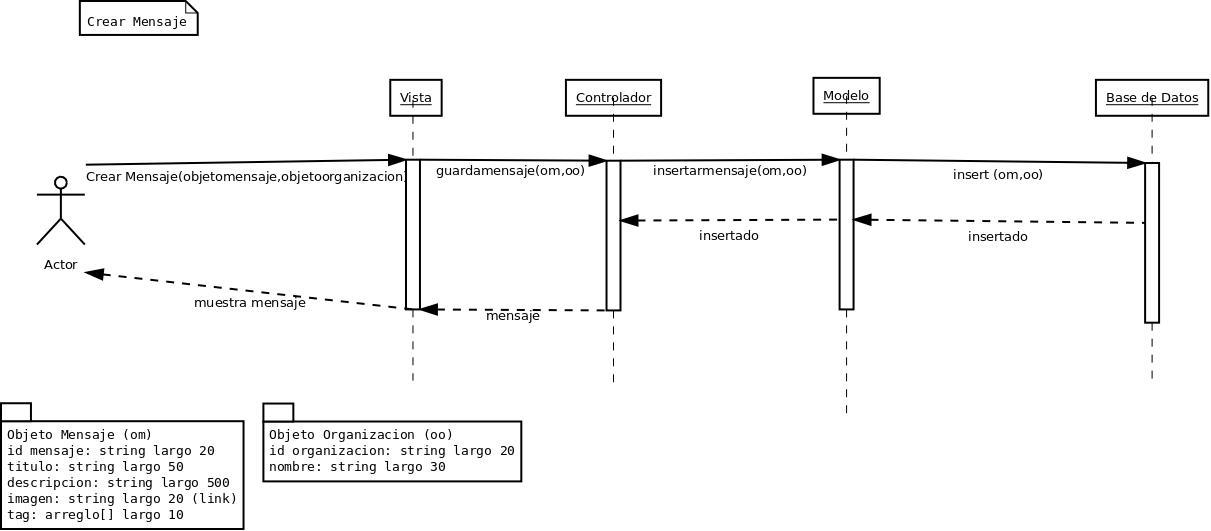
\includegraphics[scale=0.25]{/home/ijara/Dropbox/TESIS/Diagramas/diagramasdeflujo/crearmensaje.png}
\caption{Crear Mensaje}
\label{}
\end{figure}
\begin{figure}[htp]
\centering
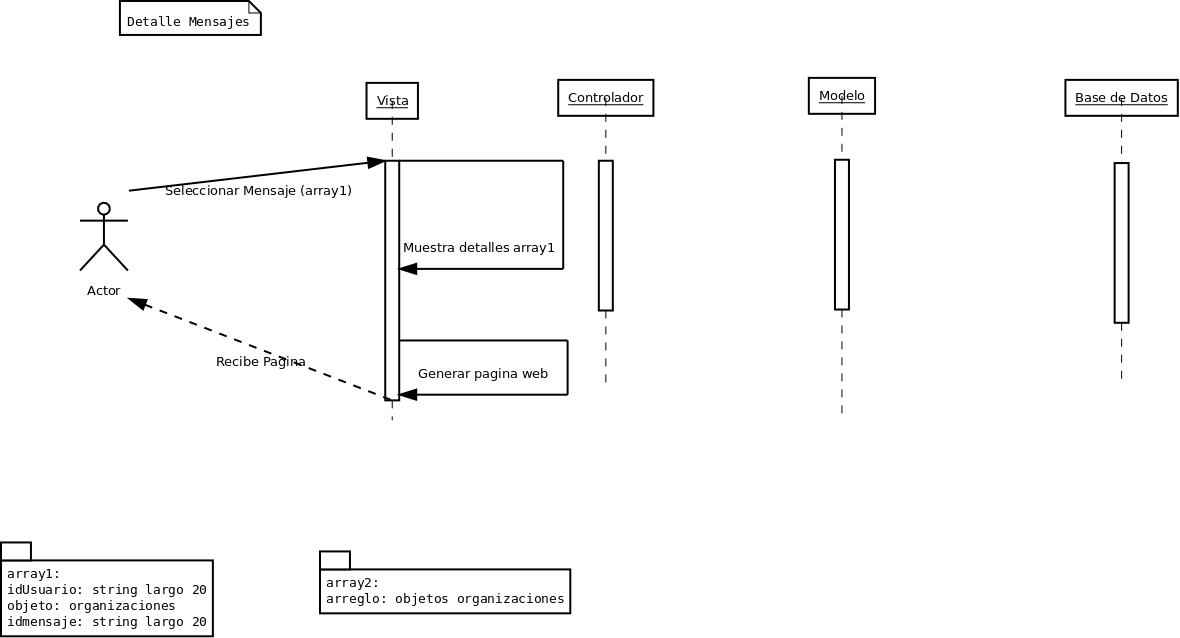
\includegraphics[scale=0.25]{/home/ijara/Dropbox/TESIS/Diagramas/diagramasdeflujo/detallemensajes.png}
\caption{Detalle Mensajes}
\label{}
\end{figure}
\begin{figure}[htp]
\centering
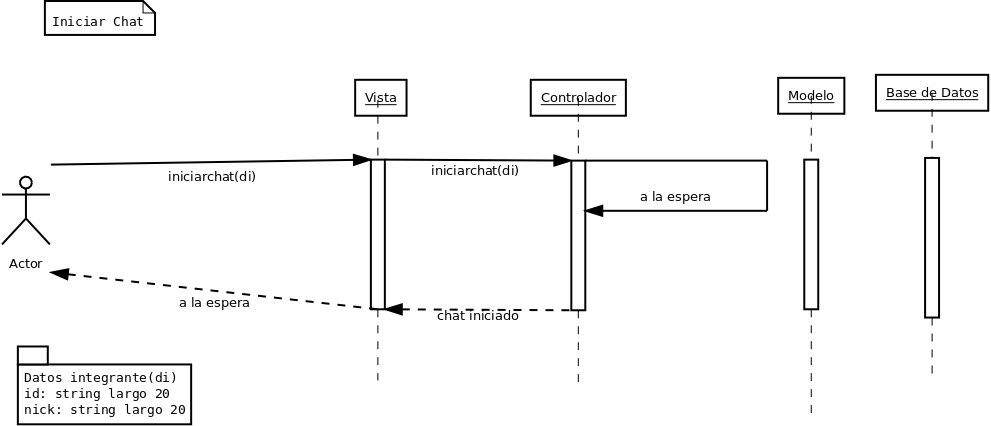
\includegraphics[scale=0.25]{/home/ijara/Dropbox/TESIS/Diagramas/diagramasdeflujo/iniciarchat.png}
\caption{Iniciar Chat}
\label{}
\end{figure}
\begin{figure}[htp]
\centering
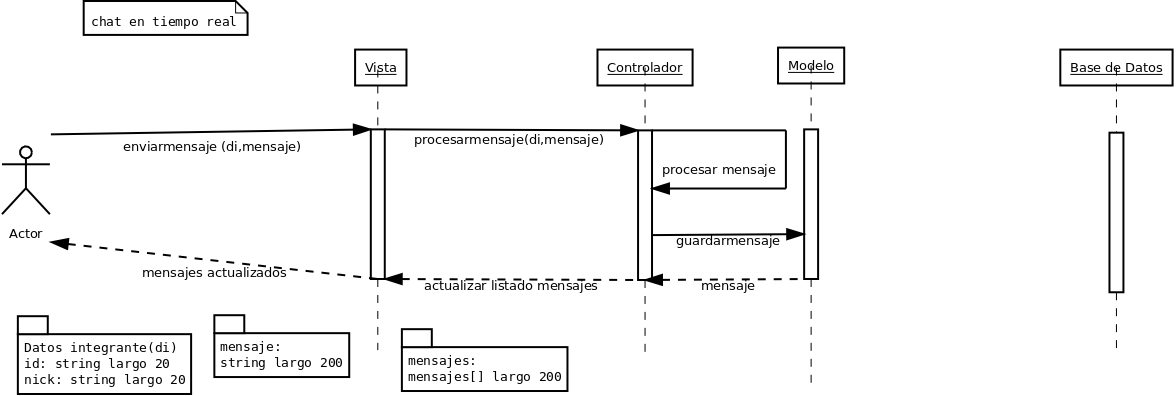
\includegraphics[scale=0.25]{/home/ijara/Dropbox/TESIS/Diagramas/diagramasdeflujo/chatentiemporeal.png}
\caption{Chat en tiempo real}
\label{}
\end{figure}
\begin{figure}[htp]
\centering
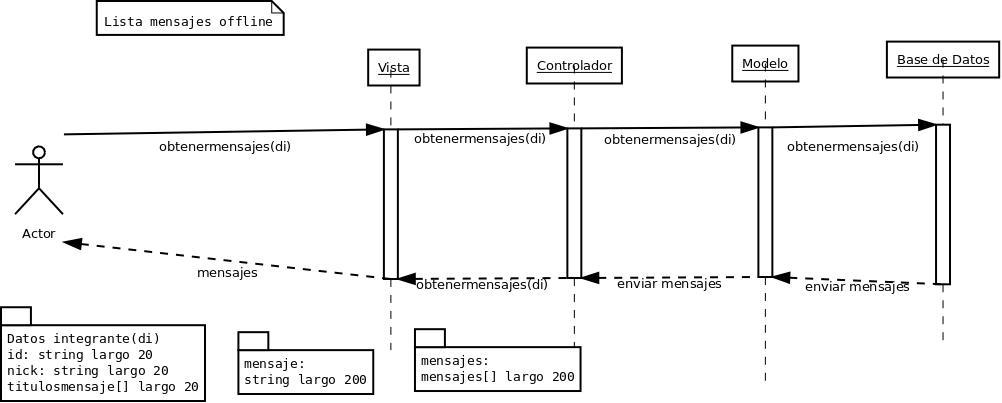
\includegraphics[scale=0.25]{/home/ijara/Dropbox/TESIS/Diagramas/diagramasdeflujo/listamensajesoffiline.png}
\caption{Lista Mensajes Offline}
\label{}
\end{figure}
\begin{figure}[htp]
\centering
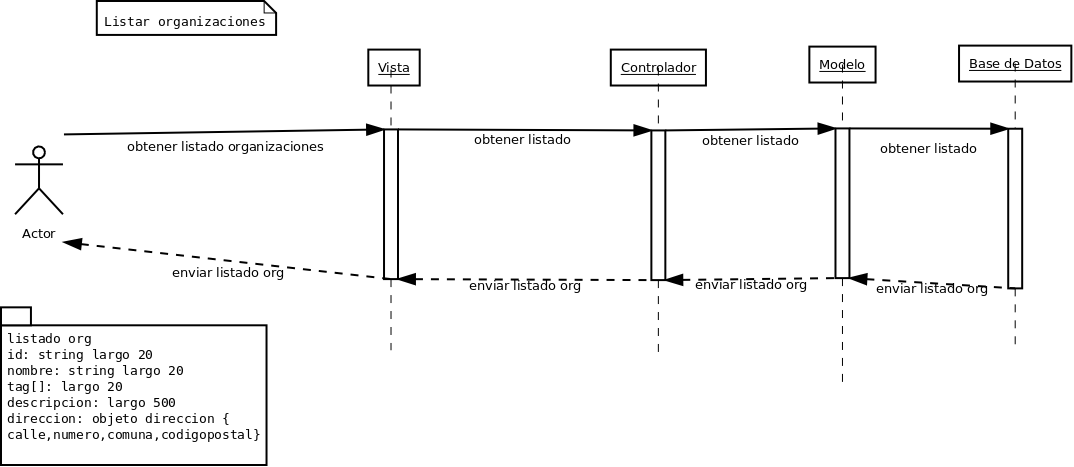
\includegraphics[scale=0.25]{/home/ijara/Dropbox/TESIS/Diagramas/diagramasdeflujo/listarorganizaciones.png}
\caption{Listar Organizaciones}
\label{}
\end{figure}
\begin{figure}[htp]
\centering
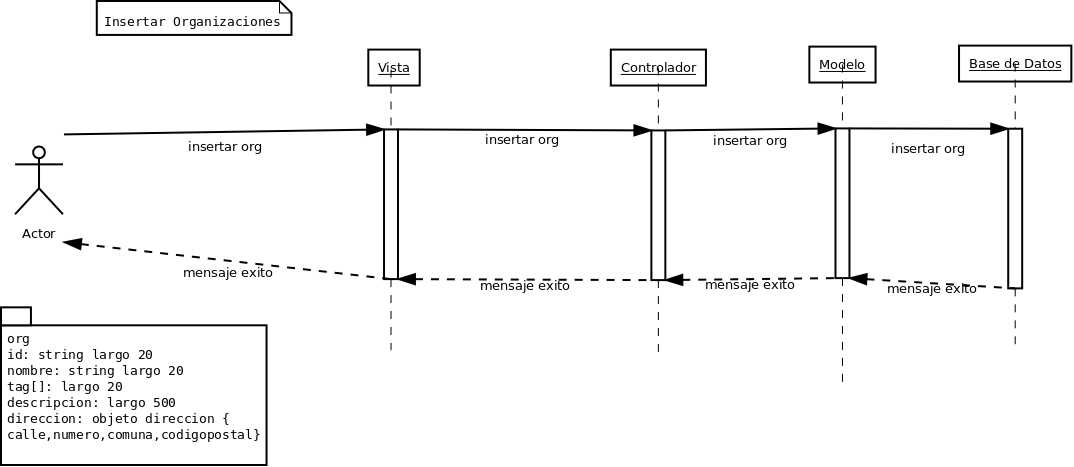
\includegraphics[scale=0.25]{/home/ijara/Dropbox/TESIS/Diagramas/diagramasdeflujo/insertarorganizaciones.png}
\caption{Insertar Organizacion}
\label{}
\end{figure}
\begin{figure}[htp]
\centering
\includegraphics[scale=0.25]{/home/ijara/Dropbox/TESIS/Diagramas/diagramasdeflujo/aceptarorechazar.png}
\caption{Aceptar o Rechazar}
\label{}
\end{figure}
\begin{figure}[htp]
\centering
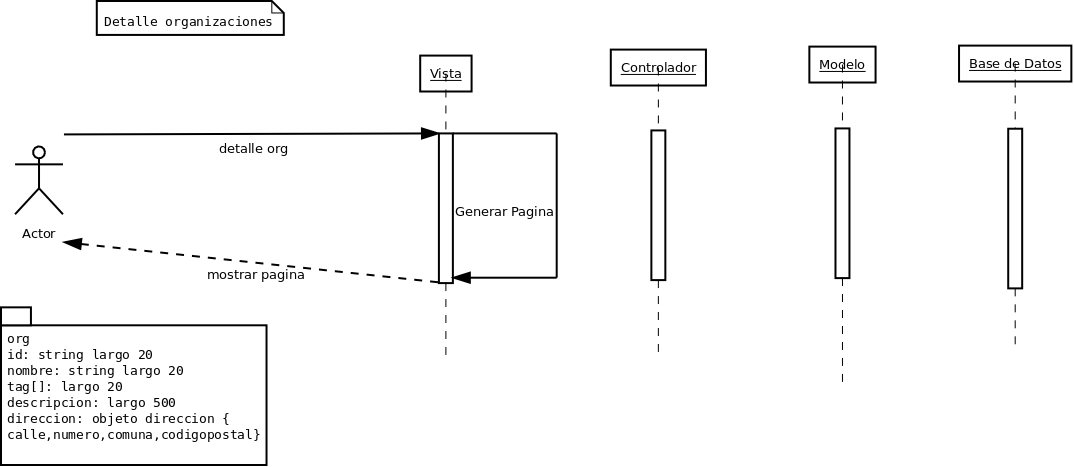
\includegraphics[scale=0.25]{/home/ijara/Dropbox/TESIS/Diagramas/diagramasdeflujo/detalleorganizaciones.png}
\caption{Detalle organizacion}
\label{}
\end{figure}
\chapter{Vistas de la aplicación}
En este capitulo se detallan las vistas que posee la aplicación web de la plataforma. En estas se puede observar como se despliegan los arreglos que entrega la plataforma web y como se distribuyen en el espacio los elementos.
\begin{figure}[htp]
\centering
\includegraphics[scale=0.50]{/home/ijara/Dropbox/TESIS/Diagramas/vistas/aceptarorechazar.png}
\caption{Aceptar o Rechazar}
\label{}
\end{figure} 
\begin{figure}[htp]
\centering
\includegraphics[scale=0.50]{/home/ijara/Dropbox/TESIS/Diagramas/vistas/borrartag.png}
\caption{Borrar Tag}
\label{}
\end{figure}
\begin{figure}[htp]
\centering
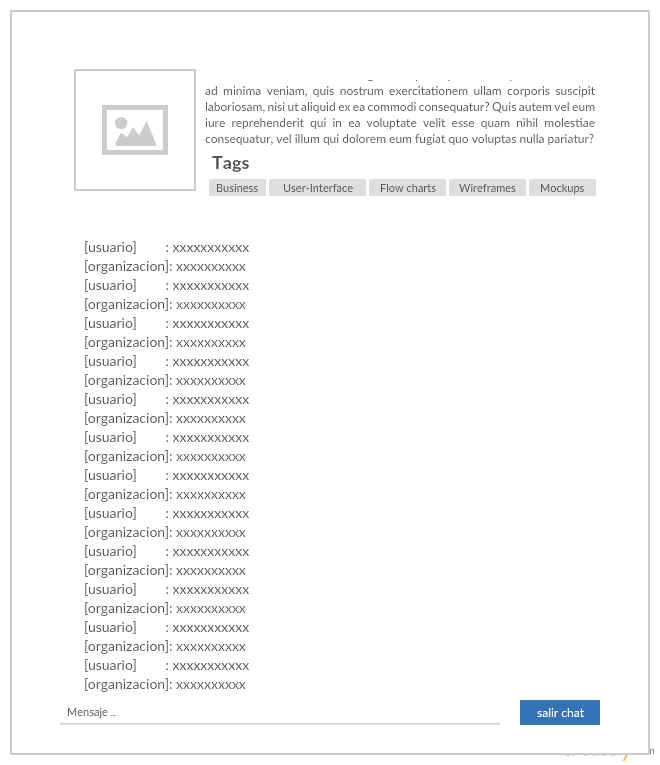
\includegraphics[scale=0.40]{/home/ijara/Dropbox/TESIS/Diagramas/vistas/chat.png}
\caption{Chat}
\label{}
\end{figure}
\begin{figure}[htp]
\centering
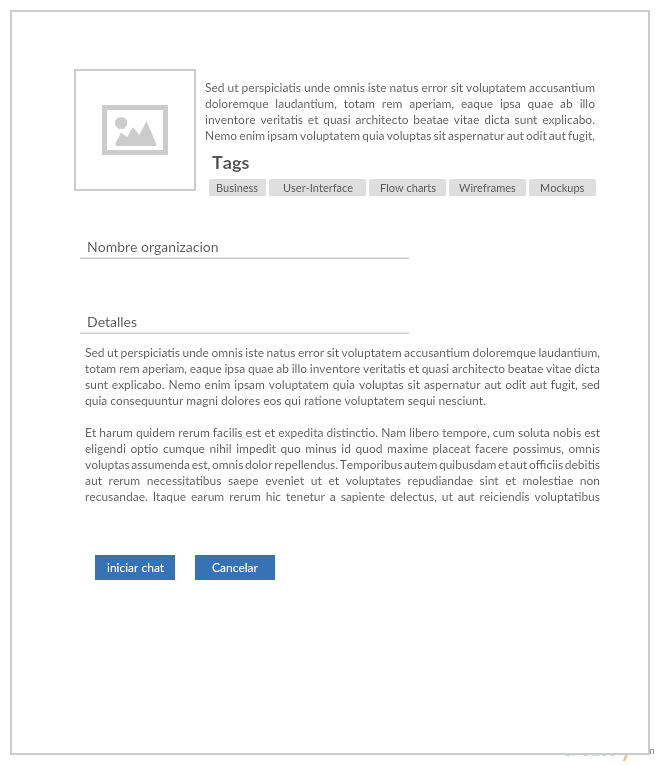
\includegraphics[scale=0.30]{/home/ijara/Dropbox/TESIS/Diagramas/vistas/detallemensaje.png}
\caption{Detalles Mensaje}
\label{}
\end{figure}
\begin{figure}[htp]
\centering
\includegraphics[scale=0.40]{/home/ijara/Dropbox/TESIS/Diagramas/vistas/editarperfil.png}
\caption{Editar Perfil}
\label{}
\end{figure}
\begin{figure}[htp]
\centering
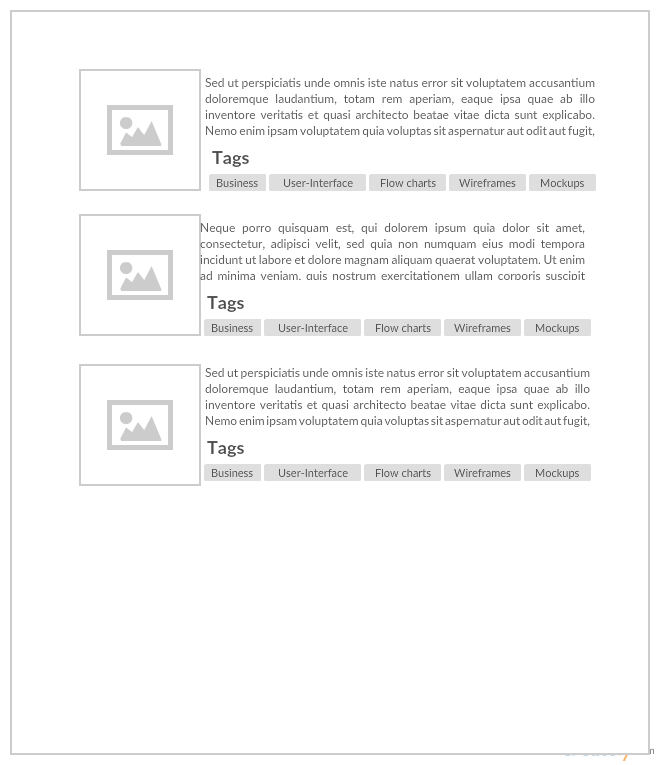
\includegraphics[scale=0.40]{/home/ijara/Dropbox/TESIS/Diagramas/vistas/index.png}
\caption{Listado Mensajes}
\label{}
\end{figure}
\begin{figure}[htp]
\centering
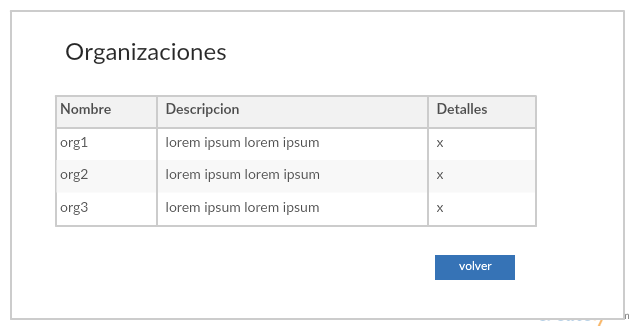
\includegraphics[scale=0.40]{/home/ijara/Dropbox/TESIS/Diagramas/vistas/listadoorganizaciones.png}
\caption{Listado Organizaciones}
\label{}
\end{figure}
\begin{figure}[htp]
\centering
\includegraphics[scale=0.40]{/home/ijara/Dropbox/TESIS/Diagramas/vistas/mostrarperfil.png}
\caption{Mostrar Perfil}
\label{}
\end{figure}
\begin{figure}[htp]
\centering
\includegraphics[scale=0.30]{/home/ijara/Dropbox/TESIS/Diagramas/vistas/seleccionartag.png}
\caption{Seleccionar Tag}
\label{}
\end{figure}
\chapter{Conclusión}
La función de desarrollar los diagramas de flujo y las vistas que tendrá nuestra aplicación es vital a la hora de desarrollar, ya que permite destacar los modulos que compondrán esta plataforma y como se relacionan entre ellos. Además de modificar y detallar como se comportarán los datos que fluyen en esta, para controlarlos y definir correctamente los requerimientos de software y hardware a utilizar en la plataforma.
Es de vital importancia desarrollar junto al cliente estos diagramas, ya que pueden aparecer nuevos requerimientos no contemplados en la etapa inicial o requerimientos que no se están llevando a cabo según el stakeholder.

\end{document}